\paragraph{\textit{Nash equilibrium and the cooperative solution.}}
The Nash equilibrium under Anticipation game also remain as in the Baseline game. We can expect a fully rational and selfish agent to always harvest seven trees at any given round to maximize his or her individual payoff as defined in equation \ref{eq:6} and \ref{eq:7}. Similarly, the Pareto optimum solution for cooperative equilibrium under Anticipation Game is also the same as in the baseline. The difference is that, in Table \ref{tab:7} under Anticipation Game, the expected value of every tree at the end of the game is now lower than four points yet remains higher than the two points participants could receive from harvesting. This means that the same socially optimum strategy persists. Except now, this increased risk causes cooperative solution to be more unstable than in the previous game to maintain. This instability arises from the fact that the decrease in future expected value per trees for society provides even more incentives for agents to harvest now rather than leaving the chance to lose out on the value that they could have received by harvesting now.
 \begin{figure}[H]
  \centering
  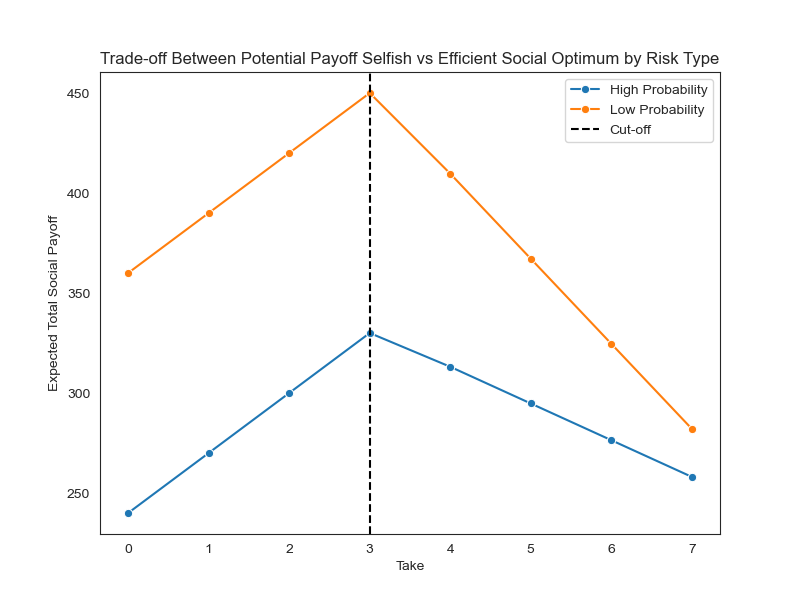
\includegraphics[width=0.6\linewidth]{../bld/graphs/0.Tradeoff2.png}
  \caption{Trade-off Between Potential Payoff Selfish vs Efficient Social Optimum}
  \label{fig:tradeoff3}
\end{figure}
 \paragraph{\textit{Expected Behaviour.}}

 Figure \ref{fig:tradeoff3} illustrates the cooperative equilibrium and the trade-off between efficiency and selfish behaviour. For any symmetric strategy that harvest any amount less than three trees is not optimal even though it is socially beneficial for everyone. Similarly, any symmetric strategy that harvest more than three trees is also not socially beneficial for everyone due to agents' selfish behaviour that strive to benefit own payoff at the expense of society. Notice that although there is an increased risk, the predicted behaviour and types do not change between Baseline and the Anticipation game as illustrated in Figure \ref{fig:tradeoff2} and \ref{fig:tradeoff3}.
